% LTeX: language=de-DE
\section{Partikelschwarmoptimierung}
Die Partikelschwarmoptimierung/particle swarm optimization (PSO) wurde zuerst von Dr. Kennedy und Dr. Eberhart in 1995 vorgestellt\cite{kennedy1942particle}.
Sie ist inspiriert vom Verhalten von Vogelschwärmen und Fischschulen. Jeder Teil wird als Partikel bezeichnet, die Gesamtheit als Schwarm.
\\ Die Partikel werden gleichverteilt über dem Suchbereich verteilt. Sie erhalten eine zufällige Startgeschwindigkeit. 
Der Suchraum hat D Dimensionen und N ist die Menge an Partikeln. Nun hat das i-te Partikel die Position $X_i=(x_{i1},x_{i2},x_{i3},...\ ...x_{iD})$
  und die Geschwindigkeit
  $V_{i}=(v_{i1},v_{i2},v_{i3},...\ ...v_{iD})$. Außerdem speichert jedes Partikel seine beste Position P\textsubscript{ibest} und erhält die insgesamt beste Position P\textsubscript{gbest}. 
\\
Jedes Partikel updated seine Position nach den folgenden Gleichungen:\\\\
\large $V_i^{k+1}=wV_i^k+c_1r_1(P_{ibest}-X_i^k)+c_2r_2(P_{gbest}-X_i^k)$
\\\\\normalsize
$X_i^{K+1}=X_i^K+V_i^{K+1}$
\begin{itemize}

  \item k: Nummer der Iteration
  \item i: Nummer des Partikels
  \item w: Startgewicht, gibt an wie stark/schwach sich die Geschwinidgkeit pro Iteration verändert, um Divergenz zu vermeiden sollte es  kleiner als 1 gewählt werden
  \item c1,c2: kognitives und soziales Gewicht, positive Konstanten
  \item $r_1,r_2$: uniform verteilte Zufallswerte im Bereich [0,1]

\end{itemize}
Schritte der gründsätzlichen Durchführung der Partikelschwarmoptimierung:
\begin{enumerate}
  \item Initialisierung: Die Partikel werden gleichverteilt initialisiert und erhalten eine Startgeschwindigkeit
  \item Evaluierung: Die Partikel werden nach einer Fitnessevaluierung ausgewertet 
  \item Update P: Der so gewonnene Fitnesswert wird dem bisher besten Fitnesswert des Partikels verglichen, ist er besser wird $P_{ibest}=P_i$. Ist dieser Wert auch besser als $P_{gbest}$ so ersetzt $P_i P_{gbest}$
  \item Update Partikel: Die Position und Geschwindigkeit werden nach den obigen Formeln verändert.
  \item Wiederholung: Schritt 2 bis 4 werden nun bis Erreichen des Abbruchkriteriums wiederholt
\end{enumerate}
Die Partikelschwarmoptimierung kann auf unterschiedliche Weisen umgesetzt werden.
Das Abbruchkriterium kann unterschiedlich gewählt werden. Standardmäßig werden hier entweder die Anzahl der Iterationen im Vorhinein festgelegt oder der Algorithmus endet nach einer zu geringen Änderung nach mehreren Iterationen. 
Um die Konvergenz zu beschleunigen, kann der $P_{ibest}$-Wert anstatt des persönlich besten Wertes den besten Wert eines bestimmten Umfelds speichern.
Der Wahl der Fitnessevaluierung kommt bei PSO ein großer Wert zukommen. Eine gut gewählte Fitnessfunktion kann die Konvergenz stark beschleunigen und somit den benötigten Rechenaufwand minimieren.\\
PSO ist einfach zu implementieren und hat nur wenige Parameter die gesetzt werden müssen. Es braucht keine skalierten Daten und ist einfach zu parallelisieren \cite{poli2007particle}.
Eine Umsetzung mit einem großen kognitiven Gewicht $c_1$ führt zu einer ausgiebigen Exploration, während ein großes soziales Gewicht $c_2$ zu einer schnellen Konvergenz führt. Daher können diese Parameter dynamisch gewählt werden, um anfangs den gesamten Suchraum zu erforschen und später trotzdem schnell zu konvergieren \cite{suganthan1999particle}. 
Umsetzungen von PSO lassen sich in zwei Kategorien einteilen: synchrone (S-PSO) und asynchone (A-PSO) Partikelschwarmoptimierung. Im ursprünglichen, asynchronen PSO wurden die Geschwindigkeiten und Positionen aller Partikel gelichzeitig am Ende jeder Iteration verändert. Im asynchronen PSO wird die Geschwindigkeit und Position der Partikel dauerhaft basieren auf den verfügbaren Informationen aktualisiert.  S-PSO erreicht eine höhere Ausnutzung, während A-PSO eine besser Exploration, sowie eine schneller Konvergenz liefert. \cite{carlisle2001g}, \cite{ab2014synchronous}
PSO teilt viele Merkmale mit genetischen Algorithmen. Beide basieren auf einer zufälligen Initialisierung ihrer Agenten und entwickeln diese Anhand einer Fitnessevaluierung weiter. Allerdings erfolgt der Informationsaustausch grundlegend unterschiedlich. Während bei einem genetischen Algorithmus alle Agenten untereinander Informationen austauschen, erfolgt dies bei einer PSO nur in eine Richtung, vom besten Partikel zu allen anderen.\\

\begin{figure}
  \centering
  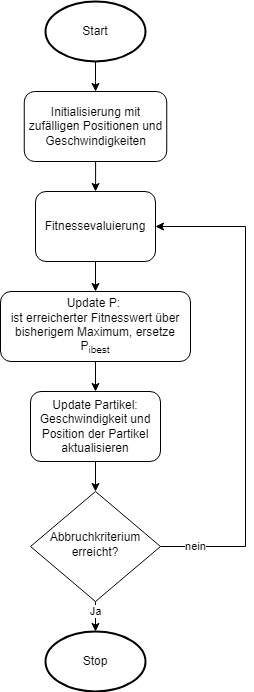
\includegraphics[scale=0.75]{Flow_PSO.png}
  \caption{Flussdiagramm von PSO}
  \label{fig:Figure_PSO}
\end{figure}

\section{Ameisen Algorithmen}
Ameisenalgorithmen sind von der Futtersuche der Ameisen abgeleitet. Ameisen kommunizieren über Stigmergie. Das heißt,sie kommunizieren nur indirekt indem sie ihre lokale Umwelt verändern. Jede Ameise scheidet auf ihrem Weg Pheromone aus, welche mit der Zeit verdunsten. 
Folgende Ameisen wählen wahrscheinlicher einen Weg mit größerer Pheromonkonzentration. 
Existieren nun zwei unterschiedlich lange Wege mit gleicher Pheromonkonzentration, entscheiden sich etwa gleich viele Ameisen für beide Wege. 
Da die Ameisen auf dem kürzeren Weg in gleicher Zeit allerdings öfter laufen, steigt hier die Konzentration schneller als auf dem längeren Weg. 
Infolgedessen laufen immer mehr Ameisen den kürzeren Weg und es bildet sich eine Ameisenstraße.\\
Es gibt viele verschiedene Umsetzungen der Ameisenalgorithmen. Der erste Ansatz wurde von Marco Dorigo 1991 vorgestellt\cite{Dorigo1991AntSA} und 1996 nochmal verbessert\cite{484436}.
Sein Ansatz namens \emph{Ant System} lieferte Grundlagen welche er 1997 in einem neuen System namens \emph{Ant Colony System} weiter verbesserte\cite{585892}. In 2000 veröffentlicht Stützle Hoos einen weiteren ACO Algorithmus namens \emph{MAX-MIN Ant System (MMAS)} \cite{STUTZLE2000889}. Es exisitieren noch einige weiter ACO Algortihmen, wie das \emph{best-worst Ant System (BWAS)}\cite{cordon2000new} oder das \emph{Hyper-Cube Ant System}\cite{blum2004hyper}. Diese sind allerdings nicht so verbreitet und werden daher im Folgenden nicht weiter behandelt. \\
Im Folgenden werden wir erst auf AS eingehen und dann die Unterschiede zu MMAS und ACS erklären.
\subsubsection{Ant System}
Jede Ameise bewegt sich von Punkt x zu Punkt y mit folgender Wahrscheinlichkeit: \\

\large$p_{xy}^k=\frac{(T_{xy}^a)(n_{xy}^b)}{\Sigma(T_{xy}^a)(n_{xy}^b) }$
\normalsize
\begin{itemize}
  \item $p_{xy}$: Wahrscheinlichkeit des Übergangs von x auf y
  \item $T_{xy}$: Menge an Pheromonen auf dem Übergang von x nach y 
  \item a: Gewicht des Einflusses von $T_{xy}$
  \item $n_{xy}$: Maß wie wünschenswert dieser Übergang ist
  \item b: Gewicht des Einflusses von $n_{xy}$
\end{itemize}

$n_{xy}$ wird berechnet durch:\\ 
\begin{large}
  $n_{xy}=\frac{1}{d_{xy}}$
\end{large}

\begin{itemize}
  \item $d_{xy}$: Abstand zwischen x und y.
\end{itemize}

Nun bewegt sich jeder Agent nach der von ihm berechneten Wahrscheinlichkeit, bis er den Zielzustand erreicht. Außerdem erhält jeder Agent eine Liste der bereits besuchten Zustände, die er nichtmehr besuchen darf, um einen Kreislauf zu verhindern. Dann werden die Pheromone folgendermaßen aktualisiert:\\\\\large
$T_{xy}^k=(1-p)T_{xy}^k+\Delta T_{xy}^k$\normalsize
\begin{itemize}
  \item p: Pheromonverdunstung
  \item k: Nummer der Ameise
  \item $\Delta T_{xy}^k$: in diesem Schritt ausgeschüttete Pheromone auf dem Schritt von x nach y
\end{itemize}
$\Delta T_{xy}^k$ berechnet sich nun folgendermaßen:\\
\large
$\Delta T_{xy}^k = \left\{
\begin{array}{ll}
\frac{Q}{L_k} & \normalsize \textrm{wenn Zustand besucht} \\
0 & \, \normalsize\textrm{sonst} \\
\end{array}
\right. $
\normalsize
\begin{itemize}
    \item Q: Konstanter Wert, wieviel Pheromone ein Agent ausschüttete
    \item $L_k$: Länge des Pfades der Ameise
\end{itemize}

Die Wahl der Pheromonverdunstung p hat einen großen Einfluss auf den Erfolg des Algorithmus. Er bestimmt Erkundung und Ausnutzung der Agenten. Ein zu hoher Wert führt zu zuviel Erkundung und das Verlorengehen von Ameisen. Ein zu niedriger Wert schränkt die Erkundung zusehr ein und der optimale Pfad wird unter Umständen nicht gefunden.\\
\subsubsection{MAX-MIN Ant System}
Das MAX-MIN Ant System(MMAS) wurde eingeführt um die Performance des Systems auf großen Daten zu verbessern. Gegenüber AS gibt es zwei große Unterschiede. Es gibt es einen maximalen sowie einen minimalen Wert für die Pheromonkonzentration auf einem Übergang, $T_{xy}$. Die minimal und maximal Werte $T_{min}$ und $T_{max}$ werden für ein Problem spezifisch empirisch gewählt\cite{socha2002max}. Allerdings gibt es dafür Richtlinine die bei einer guten Wahl helfen kann\cite{STUTZLE2000889}.\\
Bei MMAS kann außerdem nur der beste Agent die Pheromone verändern.\\
$\Delta T_{xy}$ wird berechnet mit:\\
\large
$\Delta T_{xy}  = \left\{
  \begin{array}{ll}
  \frac{1}{L_{best}} & \normalsize\textrm{wenn Übergang benutzt} \\
  0 & \, \normalsize \textrm{sonst} \\
  \end{array}
  \right. $
  \normalsize\\\\
$L_{best}$ kann jetzt entweder der beste bisherige Pfad,der beste Pfad aus der letzten Iteration sein oder eine Kombination der beiden.\\
\subsubsection{Ant Colony System }
Ant Colony System (ACS) bringt mehrere kleinere Verbesserungen mit sich. Die wichtigste Veränderung ist die Erweiterung des Pheromonupdates. Diese wird nun in zwei Schritten vorgenommen. Der erste Schritt ist das lokale Pheromonupdate. Jeder Agent aktualisiert nach jedem Schritt die Pheromone auf seinem letzten Übergang mit folgender Gleichung:\\\\

\begin{large}
  $T_{xy}=(1-\varphi)\cdot T_{xy}+\varphi\cdot T_0$\\
\end{large}

\begin{itemize}
  \item $\varphi$: Pheromon-Verdunstungskoeefizient, Wert zwischen 0 und 1
  \item $T_0$: Initialer Wert des Pheromons
\end{itemize}
Das Ziel des lokalen Updates ist die Erweiterung der Suche in einer Iteration. Durch das Vermindern der Konzentration an bereits besuchten Übergängen werden folgende Agenten begünstigt, andere Übergänge zu wählen und somit andere Lösung zu erzeugen. Dies vermindert die Überlagerung von gleichen Lösungen, welche aufgrund der Updates nur mit den besten Lösungen unerwünscht wird\cite{dorigo1997ant}. Die zweite Updateregel, das Offline Pheromon Update wird wie bei MMAS mit dem besten Pfad insgesamt oder dem besten Pfad der Iteration durchgeführt. Die Formel ist nur leicht abgeändert: \\\\

\begin{large}
  $T_{xy}  = \left\{
  \begin{array}{ll}
  (1-p)\cdot T_{xy}+p\cdot \Delta T_{xy} & \normalsize \textrm{wenn Übergang auf dem besten Pfad} \\
  T_{xy} & \, \normalsize \textrm{sonst} \\
  \end{array}
\right. $  
\end{large}


Ein weiterer Unterschied ist die Nutzung einer pseudorandomisierten Auswahl. Ist die Wahrscheinlichkeit einen Pfad zu wählen über einem gewählten Schwellwert, so wird der Agent definitiv diesen Pfad wählen. Durch die Abnutzung der besuchten Pfade kann dies nun genutzt werden, um die Suche zielgerichteter zu gestalten, ohne die anderen Pfade komplett auszuschließen\cite{gambardella1996solving}.\\

Schritte der grundsätzlichen Durchführung von ACO:
\begin{enumerate}
  \item Initialisierung: Die Übergänge zwischen Start und Ziel bekommen einen Wert für n zugewiesen
  \item Jede Einheit bewegt sich einen Schritt übereinstimmend mit der berechneten Wahrscheinlichkeit.  Wiederholen, bis das Ziel erreicht ist
  \item Die Länge der Pfade messen und Pheromonkonzentration aktualisieren
  \item Die Länge aller Pfade mit dem bisherigen besten Pfad vergleichen, den besten Pfad speichern
  \item Wiederholung: Schritt 2-4 wiederholen bis Abbruchkriterium erreicht ist
\end{enumerate}

\begin{figure}
  \centering
  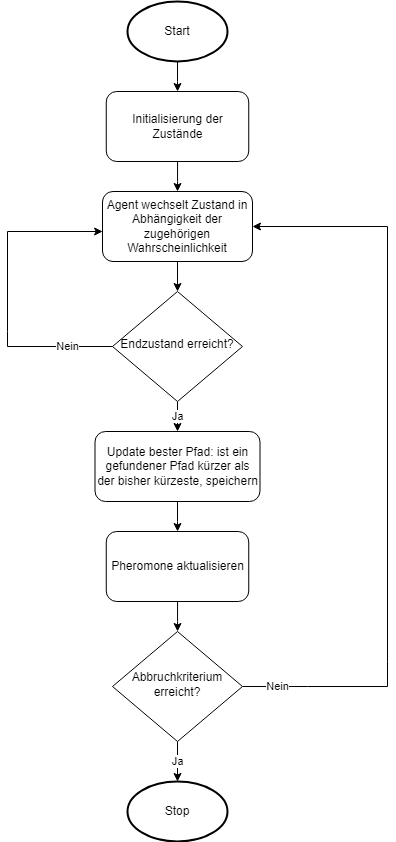
\includegraphics[scale=0.75]{Flow_ACO.png}
  \caption{Flussdiagramm von ACO}
  \label{fig:Figure_ACO}
\end{figure}

\section{Bienen Algorithmen}
Der Bienen Algorithmus ist von der Futtersuche der Bienen abgeleitet.ABC wurde in 2005 von Karaboga vorgestellt\cite{karaboga2005idea}. Ein kleiner Teil des Bienenschwarms fungiert als Kundschafter für die Kolonie.
Sie sind konstant zufällig auf der Futtersuche. Finden sie eine Futterquelle analysieren sie deren Effektivität und kehren zum Bienenstock zurück. Die Effektivität hängt von Faktoren wie der Menge, Entfernung und Zuckergehalt ab.\cite{PHAM2006454}
Die Bienen, die eine effektive Futterquelle gefunden haben, führen nun einen sogenannten \emph{waggle dance} auf dem \emph{dance floor} aus \cite{Seeley+1995}. Damit gibt sie die Wegbeschreibung zur Futterquelle weiter.
Unbeschäftigte Arbeiterbienen schauen auf dem dance floor nach Wegbeschreibungen. Umso effektiver die Futterquelle, umso länger der Tanz, daher werden auch mehr Arbeiterbienen diese ausnutzen.\cite{KARABOGA2009108} ABC ereicht gute Resultate für relativ niedrige Rechenaufwände \cite{karaboga2008performance}. Außerdem hat es nur sehr wenige Kontrollparameter die gewählt werden müssen.\\

Im Artificial Bee Colony (ABC) Algorithmus gibt es drei Gruppen an Bienen:
\begin{enumerate}
  \item Kundschafter (Scout) Bienen: Sie fliegen zufällig auf der Futtersuche umher
  \item Betrachtende Bienen: Sie stehen am dance floor und beobachten die Tänze. Sie suchen sich den besten aus und werden nun zu beschäftigten Bienen
  \item Beschäftigte Bienen: Sie fliegen zu der von ihr gewählten Futterquelle. Nachdem sie zurückgekehrt sind kommunizieren sie ihre Informationen auf dem dance floor weiter
\end{enumerate} 
Die Position einer Futterquelle repräsentiert eine mögliche Lösung des Optimierungsproblems, die Effektivität der Futterquelle die damit verbundene Fitness.
Jede beschäftige Biene ist mit einer Lösung verknüpft. Das heißt, es gibt gleich viele beschäftigte Bienen wie Futterquellen.\cite{ pham2005bees} Ist eine Futterquelle erschöpft, so werden die damit verknüpften beschäftigten Bienen zu betrachtenden Bienen. Dies wird im Algorithmus durch einen Parameter $limit$ umgesetzt. Für jede Lösung wird eine Versuchsanzahl pro Iteration hochgezählt, erreicht diese den $limit$-Wert wird die Lösung nichtmehr weiter besucht und die Agenten suchen sich neue Lösungen.
\\
Der Algorithmus beginnt mit der Initialisierungphase. Es werden zufällige Futterquellen nach folgender Formel initialisiert: \\\\\large
$x_{m,i}=l_i+r \cdot (u_i-l_i)$
\normalsize
\begin{itemize}
  \item $x_{m,i}$: Der Wert von m in der Dimension i
  \item $l_i$: unterer, beziehungsweise oberer Rand von $x_{m,i}$
  \item r: zufälliger Wert im Bereich [0,1]
\end{itemize}

Die Fitnesswerte der so erhaltenen Lösungen werden evaluiert und gespeichert.\\
Dann kommt die Phase der beschäftigten Bienen.
Die beschäftigten Bienen suchen eine bessere Futterquelle/Lösung in der Nähe ihrer Quelle ($x_m$) nach folgender Gleichung: \\\\\large
$v_{m,i}= x_{m,i}+\Phi _{m,i}( x_{m,i}- x_{k,i})$
\normalsize
\begin{itemize}
  \item $x_k$: zufällig gewählte Futterquelle
  \item i: zufällige Dimension
  \item $\Phi _{m,i}$: zufällige Zahl im Bereich [-1,1]
\end{itemize}

Nun wird die Fitness von $v_{m}$ evaluiert, ist sie besser als $x_m$ ersetzt $v_m$ $x_m$ als Futterquelle.\\
Nun folgt die Phase der Beschäftigten Bienen. Sie bekommen die Futterquellen der Beschäftigten Bienen sowie deren Fitnessevaluierung.  Nun wählen sie eine Futterquelle abhängig von folgender Wahrscheinlichkeit:\\\\ 
\large
$p_i=\frac{f_i}{\Sigma^N_{n=0}f_n}$
\normalsize
\begin{itemize}
  \item $f_i$: Fitness des Lösung
  \item N: Anzahl aller Lösungen
\end{itemize}
Auch hier wird die Fitness des erhaltenen Wertes evaluiert und im Falle einer Verbesserung der alte Wert ersetzt.\\
In der Kundschafter Bienen Phase werden die Anzahl der Versuche einer Quelle überprüft. Wurde die Futterquelle schon öfter erfolglos versucht zu optimieren, wie der $limit$ Parameter vorgibt, so wird die damit verknüpfte beschäftigte Biene eine Kundschafter Biene. Kundschafter Bienen benutzen die Formel aus der Initialisierung, um zufällige Lösungen zu suchen und zu evaluieren. Treffen sie so  zufällig auf eine Lösung mit einem guten Fitnesswert, so werden sie die beschäftigte Biene dieser Lösung.\\
Eine verbesserte Umsetzung für ABC wurde im Jahr 2014 von Karaboga veröffentlicht. Die quick Artificial Bee Colony (qABC) verändert das Verhalten der betrachtenden Bienen, um diese der realen Welt besser anzupassen und die Optimierung zu verschnellern. In der echten Welt, bekommen die betrachtenden Bienen nur eine Region durch den waggle dance mitgeteilt, und suchen sich dort die für sie beste Option zum Ausnutzen. Bei der normalen Umsetzung von ABC wird allerdings die gleiche Formel zugrunde gelegt. Daher führt der qABC Algorithmus folgende Formel für die betrachtenden Bienen ein:\\\\\large
$v_{m,i^{best}}= x_{m,i^{best}}+\Phi_{m,i}( x_{m,i^{best}}- x_{k,i})$
\normalsize
\begin{itemize}
  \item $x_{m,i^{best}}$: beste gefundene Lösung in der Nachbarschaft
\end{itemize}

Das heißt, die betrachtenden Bienen bekommen von den beschäftigten Bienen einen Punkt, welchen sie als Mittelpunkt für eine Nachbarschaft wählen. Dann suchen sie in dieser Nachbarschaft den für sie besten Punkt und errechnen den dazugehörige Fitnesswert. Um die Größe der Nachbarschaft zu bestimmen, wird der Parameter r eingeführt, welcher der Radius der Nachbarschaft angibt. Bei einem Radius r=0 wird der qABC wieder zu einem standartmäßigen ABC.
\\
Schritte der gründsätzlichen Durchführung des Bienen Algorithmus:
\begin{enumerate}
  \item Initialisierung: Initiale Lösungen werden gewählt 
  \item Fitness der initialen Lösungen berechnen
  \item Jeder Lösung wird eine beschäftigte Biene zugewiesen,sie sucht in der Umgebung nach einer besseren Lösung
  \item Ihre Lösung wird evaluiert und, wenn besser als die bisherige, gespeichert
  \item Jede betrachtende Biene wählt eine Lösung, sie sucht in der Umgebung nach einer besseren Lösung
  \item Ihre Lösung wird evaluiert und, wenn besser als die bisherige, gespeichert
  \item Kundschafter Bienen suchen zufällig nach neuen Lösungen
  \item Ihre Lösung wird evaluiert und, wenn ähnlich gut wie bisherige, gespeichert
  \item Wiederholung: Schritt 2-8 wiederholen bis Abbruchkriterium erreicht ist
\end{enumerate}

\begin{figure}
  \centering
  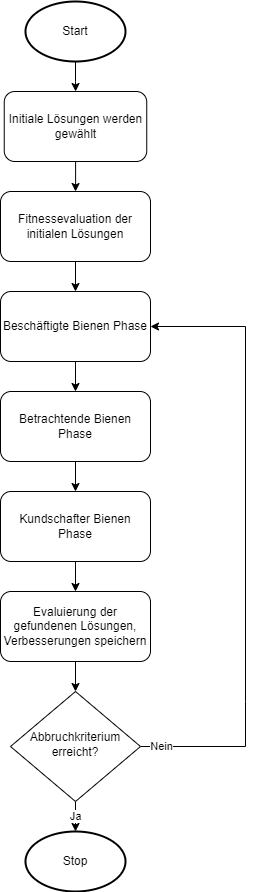
\includegraphics[scale=0.75]{Flow_ABC.png}
  \caption{Flussdiagramm von ABC}
  \label{fig:Figure_ABC}
\end{figure}